\documentclass[]{article}
\usepackage{lmodern}
\usepackage{amssymb,amsmath}
\usepackage{ifxetex,ifluatex}
\usepackage{fixltx2e} % provides \textsubscript
\ifnum 0\ifxetex 1\fi\ifluatex 1\fi=0 % if pdftex
  \usepackage[T1]{fontenc}
  \usepackage[utf8]{inputenc}
\else % if luatex or xelatex
  \ifxetex
    \usepackage{mathspec}
  \else
    \usepackage{fontspec}
  \fi
  \defaultfontfeatures{Ligatures=TeX,Scale=MatchLowercase}
\fi
% use upquote if available, for straight quotes in verbatim environments
\IfFileExists{upquote.sty}{\usepackage{upquote}}{}
% use microtype if available
\IfFileExists{microtype.sty}{%
\usepackage{microtype}
\UseMicrotypeSet[protrusion]{basicmath} % disable protrusion for tt fonts
}{}
\usepackage[margin=1in]{geometry}
\usepackage{hyperref}
\hypersetup{unicode=true,
            pdftitle={Estimating yield as a function of chill accumulation},
            pdfauthor={Katja Schiffersa, Cory Whitneya, Eduardo Fernandeza and Eike Luedelinga   aINRES-Horticultural Sciences, University of Bonn, Auf dem Huegel 6, 53121 Bonn, Germany},
            pdfborder={0 0 0},
            breaklinks=true}
\urlstyle{same}  % don't use monospace font for urls
\usepackage{graphicx,grffile}
\makeatletter
\def\maxwidth{\ifdim\Gin@nat@width>\linewidth\linewidth\else\Gin@nat@width\fi}
\def\maxheight{\ifdim\Gin@nat@height>\textheight\textheight\else\Gin@nat@height\fi}
\makeatother
% Scale images if necessary, so that they will not overflow the page
% margins by default, and it is still possible to overwrite the defaults
% using explicit options in \includegraphics[width, height, ...]{}
\setkeys{Gin}{width=\maxwidth,height=\maxheight,keepaspectratio}
\IfFileExists{parskip.sty}{%
\usepackage{parskip}
}{% else
\setlength{\parindent}{0pt}
\setlength{\parskip}{6pt plus 2pt minus 1pt}
}
\setlength{\emergencystretch}{3em}  % prevent overfull lines
\providecommand{\tightlist}{%
  \setlength{\itemsep}{0pt}\setlength{\parskip}{0pt}}
\setcounter{secnumdepth}{0}
% Redefines (sub)paragraphs to behave more like sections
\ifx\paragraph\undefined\else
\let\oldparagraph\paragraph
\renewcommand{\paragraph}[1]{\oldparagraph{#1}\mbox{}}
\fi
\ifx\subparagraph\undefined\else
\let\oldsubparagraph\subparagraph
\renewcommand{\subparagraph}[1]{\oldsubparagraph{#1}\mbox{}}
\fi

%%% Use protect on footnotes to avoid problems with footnotes in titles
\let\rmarkdownfootnote\footnote%
\def\footnote{\protect\rmarkdownfootnote}

%%% Change title format to be more compact
\usepackage{titling}

% Create subtitle command for use in maketitle
\providecommand{\subtitle}[1]{
  \posttitle{
    \begin{center}\large#1\end{center}
    }
}

\setlength{\droptitle}{-2em}

  \title{Estimating yield as a function of chill accumulation}
    \pretitle{\vspace{\droptitle}\centering\huge}
  \posttitle{\par}
    \author{Katja Schiffers\textsuperscript{a}, Cory Whitney\textsuperscript{a},
Eduardo Fernandez\textsuperscript{a} and Eike
Luedeling\textsuperscript{a} \textsuperscript{a}INRES-Horticultural
Sciences, University of Bonn, Auf dem Huegel 6, 53121 Bonn, Germany}
    \preauthor{\centering\large\emph}
  \postauthor{\par}
    \date{}
    \predate{}\postdate{}
  
\usepackage{booktabs}
\usepackage{longtable}
\usepackage{array}
\usepackage{multirow}
\usepackage{wrapfig}
\usepackage{float}
\usepackage{colortbl}
\usepackage{pdflscape}
\usepackage{tabu}
\usepackage{threeparttable}
\usepackage{threeparttablex}
\usepackage[normalem]{ulem}
\usepackage{makecell}
\usepackage{xcolor}

\begin{document}
\maketitle

Data is often limited for assessing the relationship between
temperatures and yield. Here we show how, despite this lack of data, we
may still be able to make assessments and produce useful projections for
farmers and decision makers. With the right tools this data limitation
does not need to hinder our abilities to assess the relationships
between temperature and yield. For coarse assessments a lot of data may
not be necessary. We use the pasitR package (Schiffers et al., 2018) in
the R programming language (R Core Team, 2019) to illustrate methods
whereby we can embrace the inherent uncertainty in such assessments to
overcome the need for preciseness. We show a potential method for
dealing with important but also necessarily uncertain relationships in
model forecasts.

\hypertarget{yield-and-chill-data}{%
\subsection{Yield and chill data}\label{yield-and-chill-data}}

We offer an example of assessing yield given chill (Chill Portions) for
sweet cherries (\emph{Prunus avium} L.) `Lapins' and `Brooks' varieties.
We applied procedures from the \texttt{pasitR} library for estimating
yield as a function of chill accumulation (Schiffers et al., 2018). The
data was provided by the experimental orchard of the School of Agronomy
at the Pontificia Universidad Catolica de Valparaiso (Table 1). We used
weather data obtained from a local weather station (Table 2).

We used the \texttt{tempResponse\_daily\_list} in the \texttt{chillR}
package (Luedeling, 2019) to compute the chill accumulation for each
season. We defined the chilling season as the period between
1\textsuperscript{st} of May and 31\textsuperscript{st} of August (Table
3).

\begin{table}

\caption{\label{tab:tables_1_3}Yield records (in tons per hectare) for 8 seasons (2010 to 2017) for two sweet cherry cultivars (Lapins and Brooks).}
\centering
\begin{tabular}[t]{r|l|r}
\hline
Year & Variety & Yield\\
\hline
2010 & Lapins & 16.387600\\
\hline
2011 & Lapins & 11.401600\\
\hline
2012 & Lapins & 1.599200\\
\hline
2013 & Lapins & 13.521200\\
\hline
2014 & Lapins & 21.648480\\
\hline
2015 & Lapins & 9.413200\\
\hline
2016 & Lapins & 24.974440\\
\hline
2017 & Lapins & 8.515682\\
\hline
2010 & Brooks & 6.412400\\
\hline
2011 & Brooks & 1.296000\\
\hline
2012 & Brooks & 1.032000\\
\hline
2013 & Brooks & 3.396800\\
\hline
2014 & Brooks & 6.872400\\
\hline
2015 & Brooks & 2.887160\\
\hline
2016 & Brooks & 9.217320\\
\hline
2017 & Brooks & 9.892581\\
\hline
\end{tabular}
\end{table}

\begin{table}

\caption{\label{tab:tables_1_3}Weather data from a weather station placed in the orchard.}
\centering
\begin{tabular}[t]{r|l|r|r|r|r|r|r}
\hline
YEARMODA & Weather\_Station & Year & Month & Day & JDay & Tmin & Tmax\\
\hline
20100101 & Quillota & 2010 & 1 & 1 & 1 & 6.2 & 31.0\\
\hline
20100102 & Quillota & 2010 & 1 & 2 & 2 & 7.6 & 29.4\\
\hline
20100103 & Quillota & 2010 & 1 & 3 & 3 & 12.2 & 23.2\\
\hline
20100104 & Quillota & 2010 & 1 & 4 & 4 & 8.0 & 24.0\\
\hline
20100105 & Quillota & 2010 & 1 & 5 & 5 & 8.0 & 26.5\\
\hline
20100106 & Quillota & 2010 & 1 & 6 & 6 & 9.0 & 27.0\\
\hline
20100107 & Quillota & 2010 & 1 & 7 & 7 & 8.5 & 24.0\\
\hline
20100108 & Quillota & 2010 & 1 & 8 & 8 & 7.0 & 28.0\\
\hline
20100109 & Quillota & 2010 & 1 & 9 & 9 & 8.0 & 28.0\\
\hline
20100110 & Quillota & 2010 & 1 & 10 & 10 & 8.0 & 24.0\\
\hline
\end{tabular}
\end{table}

\begin{table}

\caption{\label{tab:tables_1_3}Computed chill accumulation for each pre-defined chilling season between May 1 and August 31.}
\centering
\begin{tabular}[t]{l|r|r|r|r|r}
\hline
Season & End\_year & Season\_days & Data\_days & Perc\_complete & Chill\_Portions\\
\hline
2009/2010 & 2010 & 123 & 123 & 100 & 68.45256\\
\hline
2010/2011 & 2011 & 123 & 123 & 100 & 60.46397\\
\hline
2011/2012 & 2012 & 123 & 123 & 100 & 44.61716\\
\hline
2012/2013 & 2013 & 123 & 123 & 100 & 52.14200\\
\hline
2013/2014 & 2014 & 123 & 123 & 100 & 54.60832\\
\hline
2014/2015 & 2015 & 123 & 123 & 100 & 43.24068\\
\hline
2015/2016 & 2016 & 123 & 123 & 100 & 53.47477\\
\hline
2016/2017 & 2017 & 123 & 123 & 100 & 53.95999\\
\hline
\end{tabular}
\end{table}

We developed the \texttt{chillscatter} function to create a scatter plot
of chill and yield (Fig. \ref{fig:chillscatter}). The function
calculates the associated estimated densities with loess smooth linear
fits density curves using the \texttt{scatter.hist} function in the
\texttt{plyr} package (Wickham, 2019).

\begin{figure}
\centering
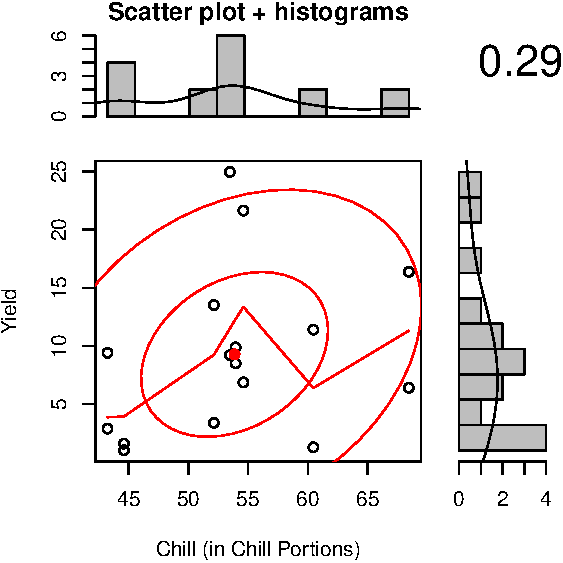
\includegraphics{Full_SHE_Chill_Yield_Model_files/figure-latex/chillscatter-1.pdf}
\caption{\label{fig:chillscatter}Scatter plot of Chill Portions (x) and
yield (y) for sweet cherries.}
\end{figure}

We developed the \texttt{chillkernel} function to perform a
two-dimensional kernel density estimation for yield and chill using the
\texttt{kde2d} function in the \texttt{MASS} package (Ripley, 2019). The
density function restricts the shape of the kernel to a bi-variate
normal kernel, so this looks slightly different compared to the scatter
plot estimates above. The plot is made with the \texttt{filled.contour}
function of the \texttt{graphics} package (R Core Team, 2019). In
\texttt{chillkernel} the density (z) over the entire plot integrates to
one, and therefore represents the relative probability of an observation
(yield along y-axis) given a specific amount of chill (along x-axis)
(Fig. \ref{fig:chillkernel}).

\begin{figure}
\centering
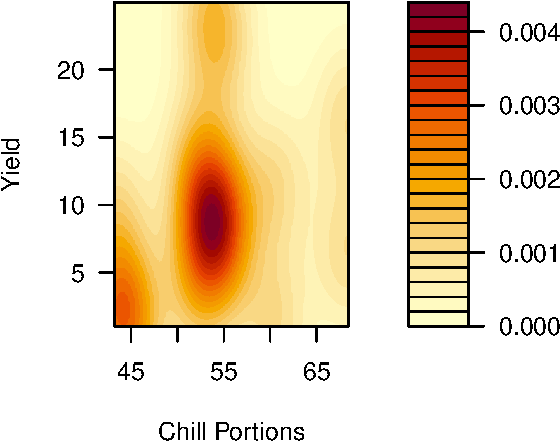
\includegraphics{Full_SHE_Chill_Yield_Model_files/figure-latex/chillkernel-1.pdf}
\caption{\label{fig:chillkernel}Density surface plot of Chill Portions
(x) and yield (y) for sweet cherries. The legend shows the value for the
estimated density (z).}
\end{figure}

\hypertarget{estimated-yield-given-the-expected-chill}{%
\subsection{Estimated yield given the expected
chill}\label{estimated-yield-given-the-expected-chill}}

We developed the \texttt{pasitR} function \texttt{chillkernelslice} to
calculate the estimated yield given the expected chill, based on a slice
of `z' from the Kernel density calculated with \texttt{chillkernel}
(Fig. \ref{fig:chillkernelslice}). The function plots the probabilities
(shown along the y-axis) for the expected yield (shown along the
x-axis). Since this is a cut through the density kernel
\texttt{chillkernel} (Fig. \ref{fig:chillkernel}), which integrates to
1, the probability values are relative, not absolute measures. We set
the value of expected chill for which to estimate yield should (the
\texttt{expectedchill} parameter) to 30.

\begin{figure}
\centering
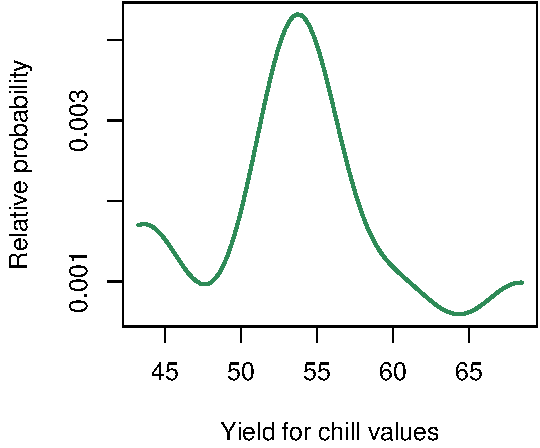
\includegraphics{Full_SHE_Chill_Yield_Model_files/figure-latex/chillkernelslice-1.pdf}
\caption{\label{fig:chillkernelslice}Estimated yield of sweet cherry
given the expected chill, based on a slice of `z' from the Kernel
density.}
\end{figure}

\hypertarget{chill-portion-intervals}{%
\subsection{Chill portion intervals}\label{chill-portion-intervals}}

We developed the \texttt{chillviolin} function to determine possible
Chill Portion intervals (Fig. \ref{fig:chillviolin}). We calculate the
optimal interval width for Chill Portions using the \texttt{IQR}
function in the \texttt{stats} package, after the Freedman-Diaconis rule
(IQR = interquartile range) (R Core Team, 2019). The
\texttt{chillviolin} function uses the \texttt{ggplot2} (Wickham et al.,
2019) library.

\begin{figure}
\centering
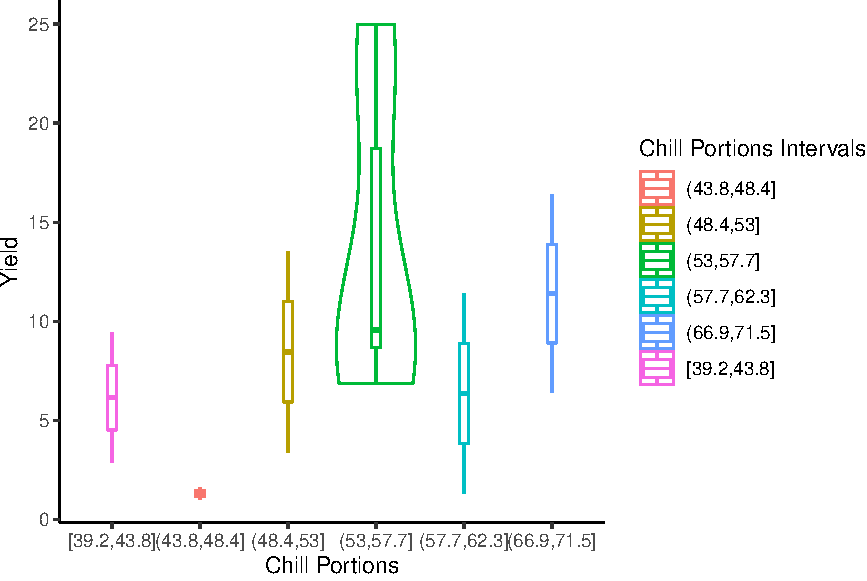
\includegraphics{Full_SHE_Chill_Yield_Model_files/figure-latex/chillviolin-1.pdf}
\caption{\label{fig:chillviolin}Violin plots with boxplot overlays of
possible Chill Portions (x) and yield (y) with six different intervals
of Chill Portions.}
\end{figure}

\hypertarget{probability-of-yield-given-chill}{%
\subsection{Probability of yield given
chill}\label{probability-of-yield-given-chill}}

We developed the \texttt{chillkernelslicerange} function to visualize
the probable yield given a likely range of expected Chill Portions (Fig.
\ref{fig:chillkernelslicerange}). The function takes the optimized
interquartile ranges for chill intervals to select a range to slice from
the density kernel \texttt{chillkernel} the same procedures we used for
a single chill value in \texttt{chillkernelslice} (Fig.
\ref{fig:chillkernelslice}). As with \texttt{chillkernelslice} the
probability values shown are relative, not absolute measures. They are
the result of cuts through the density kernel (Fig.
\ref{fig:chillkernel}), which integrates to 1.

\begin{figure}
\centering
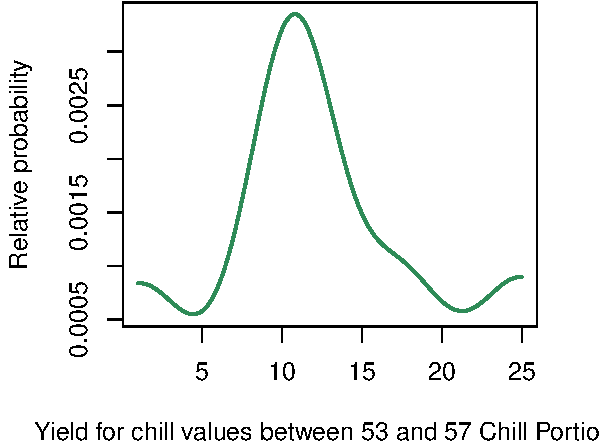
\includegraphics{Full_SHE_Chill_Yield_Model_files/figure-latex/chillkernelslicerange-1.pdf}
\caption{\label{fig:chillkernelslicerange}Probabilities (shown along the
y-axis) for the expected yield (shown along the x-axis). Here we set the
minimum Chill Portions to 53 and the maximum to 57.}
\end{figure}

\hypertarget{next-steps}{%
\section{Next steps}\label{next-steps}}

We have demonstrated the possibility for generating forecasts of
possible yields given chill. The \texttt{pasitR} functions closely
follow chillR (Luedeling, 2019) and decisionSupport (Luedeling et al.,
2019). We will continue to develop these and may integrate them into
future version of these packages. The functions are all stored in an
open access repository (\url{https://github.com/hortibonn/pasitR}) and
are free to use and modify (Schiffers et al., 2018).

\hypertarget{references}{%
\subsection*{References}\label{references}}
\addcontentsline{toc}{subsection}{References}

\hypertarget{refs}{}
\leavevmode\hypertarget{ref-R-chillR}{}%
Luedeling, E. 2019. ChillR: Statistical methods for phenology analysis
in temperate fruit trees.

\leavevmode\hypertarget{ref-R-decisionSupport}{}%
Luedeling, E., Goehring, L. and Schiffers, K. 2019. DecisionSupport:
Quantitative support of decision making under uncertainty.

\leavevmode\hypertarget{ref-R-base}{}%
R Core Team. 2019. R: A language and environment for statistical
computing. Vienna, Austria: R Foundation for Statistical Computing.

\leavevmode\hypertarget{ref-R-MASS}{}%
Ripley, B. 2019. MASS: Support functions and datasets for venables and
ripley's mass.

\leavevmode\hypertarget{ref-R-pasitR}{}%
Schiffers, K., Whitney, C., Fernandez, E. and Luedeling, E. 2018.
PasitR: Calculates common functions for the pasit project.

\leavevmode\hypertarget{ref-R-plyr}{}%
Wickham, H. 2019. Plyr: Tools for splitting, applying and combining
data.

\leavevmode\hypertarget{ref-R-ggplot2}{}%
Wickham, H., Chang, W., Henry, L., Pedersen, T.L., Takahashi, K., Wilke,
C., Woo, K. and Yutani, H. 2019. Ggplot2: Create elegant data
visualisations using the grammar of graphics.


\end{document}
